\documentclass{beamer}

\mode<presentation>
{
\usetheme{Dresden}

\setbeamercovered{transparent}
}
\usepackage{multimedia}
\usepackage[english]{babel}
\usepackage[latin1]{inputenc}
\usepackage{amsfonts}
\usepackage{amsmath}
\usepackage{mathtools}
\usepackage{listing}
\usepackage[scaled=.90]{helvet}
\usepackage{courier}
\usepackage{graphicx}
\usepackage{color}
\usepackage{subfig}
\DeclareGraphicsExtensions{.pdf,.png,.jpg,.mps}
\usepackage[absolute,overlay]{textpos}
\setlength{\TPHorizModule}{1mm}
\setlength{\TPVertModule}{1mm}
\usepackage{ragged2e}
\justifying
\usepackage{color}
\usepackage{physics}
\usepackage{mathtools}
\usepackage{amsmath}
\usepackage{bm}
\usepackage{calc}
\usepackage{listings}
\usepackage{url}
\usepackage{rotating}
%\usepackage{calrsfs}
\usepackage{amsfonts}
\usepackage[T1]{fontenc}

%%%% A NEW COMMAND TO FIX LOGO POSITION (x,y) in mm
\newcommand{\MyLogo}{%
\begin{textblock}{13}(88,74)
%  \pgfuseimage{logo}
 
\includegraphics[height=1cm, angle=0]{images/pdp2017}
\end{textblock}
} 


%%%% A NEW COMMAND TO FIX LOGO POSITION (x,y) in mm

%%%%%%%%%%%%%%%%%%%%%%%%%%%%%%%%%%%%%%%%%%%%%%%%%%%%%%%%%%%%%%%%%%%%%%%%%

\title{A Tracking Algorithm for Particle-like Moving Objects}

\author{Davide Spataro\inst{1}, Paola Arcuri\inst{1}, Alessio De Rango\inst{1}, William Spataro\inst{1}, Donato D'Ambrosio\inst{1} and Alice Mari\inst{2}}
\institute[]{\inst{1} University of Calabria, Department of Mathematics and Computer Science \and %
\inst{2} Institute for BioEngineering University of Edinburgh}
\date{PDP 2017,  St. Petersburg, Russia\\
March 5-8, 2017}

\begin{document}


\AtBeginSection[]{
  \begin{frame}
  \vfill
  \centering
  \begin{beamercolorbox}[sep=8pt,center,shadow=true,rounded=true]{title}
    \usebeamerfont{title}\insertsectionhead\par%
  \end{beamercolorbox}
  \vfill
  \end{frame}
}

\begin{frame}
\MyLogo
\MyLogo
\titlepage
\end{frame}




\section{Introduction}
%Frame----------------------------------------------------------------------------------------------------------------------------------------------------
	\begin{frame}{Motivations}
				\begin{itemize}
					\item How bacteria react to a stimulus
					\item How a drug interfere with bacteria, changing their chemiotaxis i.e. change in movements
					\item For example monitoring how good is a drug impeding communication between cancer cells.
					\item When the number of \textit{particles} is high, manual evaluation is \textbf{infisable}
					\item It is non invasive
				\end{itemize}

	\end{frame}
	
	%Frame----------------------------------------------------------------------------------------------------------------------------------------------------
		\begin{frame}{Motivations}
				\begin{figure}
					\centering
					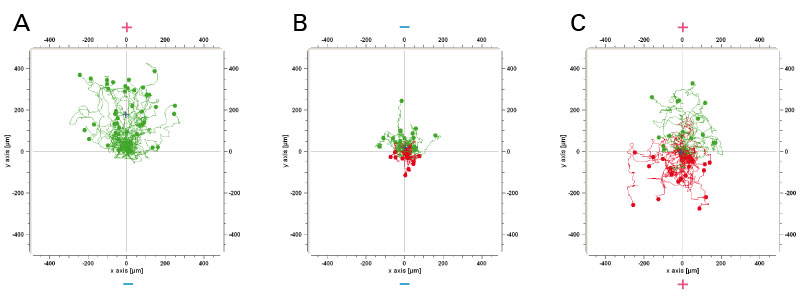
\includegraphics[scale=0.38]{./images/motivations.png}
				\end{figure}

				\begin{itemize}
					\item A: \textit{Normal} trajectories
					\item B: Drug is administred
					\item C: Red trajectories are of those who were affected by the drug
				\end{itemize}
				\textbf{Tracking allows  quantitatively analysis}!
	\end{frame}
	
%Frame----------------------------------------------------------------------------------------------------------------------------------------------------
		\begin{frame}{Motivations}
				\begin{figure}
					\centering
					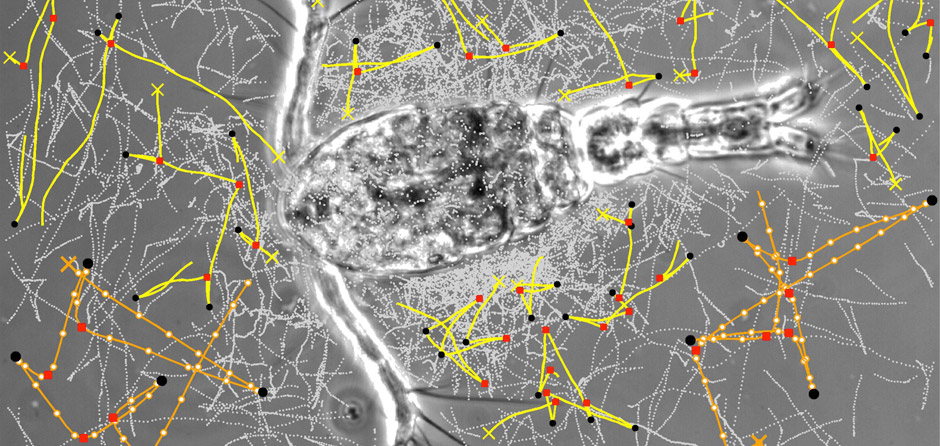
\includegraphics[scale=0.30]{./images/motivations2.png}
				\end{figure}

			

	\end{frame}
	
	
	%Frame----------------------------------------------------------------------------------------------------------------------------------------------------
		\begin{frame}{Motivations}
%				\begin{figure}
%					\centering
%					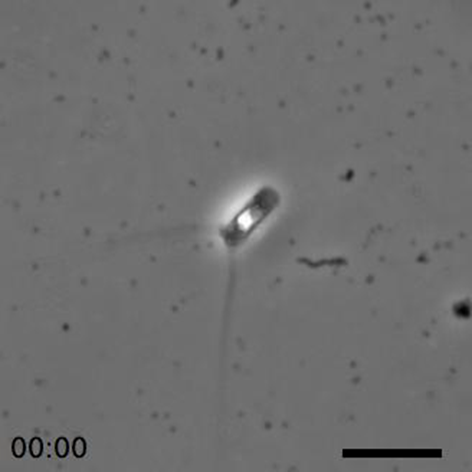
\includegraphics[scale=0.30]{./images/motivations3.png}
%				\end{figure}
\centering
\fbox{	
	\movie[width=6cm,height=6cm,autostart,loop,poster,palindrome]{}{alga.avi}}
				
	\end{frame}
	
	

\section{Image Processing Using CA}


%Frame----------------------------------------------------------------------------------------------------------------------------------------------------
		\begin{frame}{XCA - IFCA Engine - CA}
			\begin{itemize}
			\item Cellular Automata (CA) are \textbf{Turing complete dynamical system} and also a \textbf{parallel computational models} (\textit{von Neumann 1966})
			\item CA can be described as a matrix of simple processing units, the cells, each one interacting with its neighbouring ones

			\end{itemize}
					\begin{figure}
					\centering
					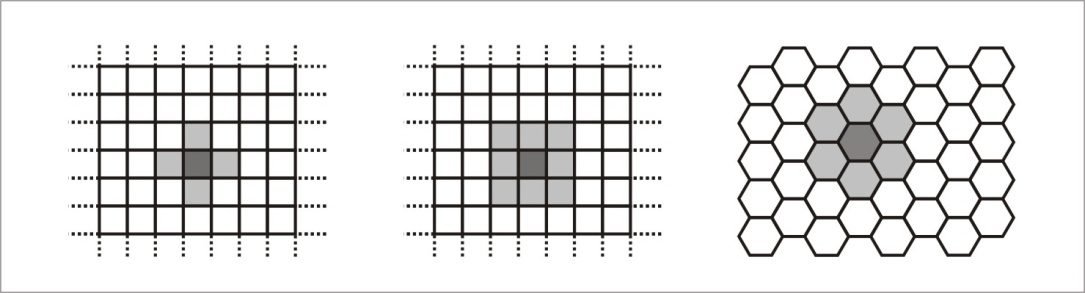
\includegraphics[scale=0.68]{./images/CA}
				\end{figure}
		\end{frame}
%Frame----------------------------------------------------------------------------------------------------------------------------------------------------
		\begin{frame}{XCA - IFCA Engine - CA}
		\[
			A = \Big<Z^d , Q, X, \tau \Big>		
		\] where:
		\begin{itemize}
		 \item $Z^d$ is the $d-$dimensional Cellular Space.
		 \item $Q$ is the \textbf{finite} set of states of the cell
		 \item $X = \{\xi_0, \xi_1, \ldots , \xi_{m-1}\}$ is the finite set of $d-$dimensional vectors that define the set of coordinates of the neighbouring cells $V(X,i)=\{i+\xi_0, i+\xi_{1},\ldots, i+\xi_{m-1}\}$

		 \item $\tau: Q^m \mapsto  Q$ is the deterministic transition function for the cell. $tau$ is applied simultaneously to each cell, for each CA step
		\end{itemize}
		\end{frame}
		
%Frame----------------------------------------------------------------------------------------------------------------------------------------------------
		\begin{frame}{XCA - IFCA Engine }
\begin{block}{A (farly large) number of Image Processing algorithm can be expressed as CA}
Convolutional filters $\mapsto$ $X$ and $\tau$ in CA's world.

\end{block}		
		
		\begin{figure}
					\centering
					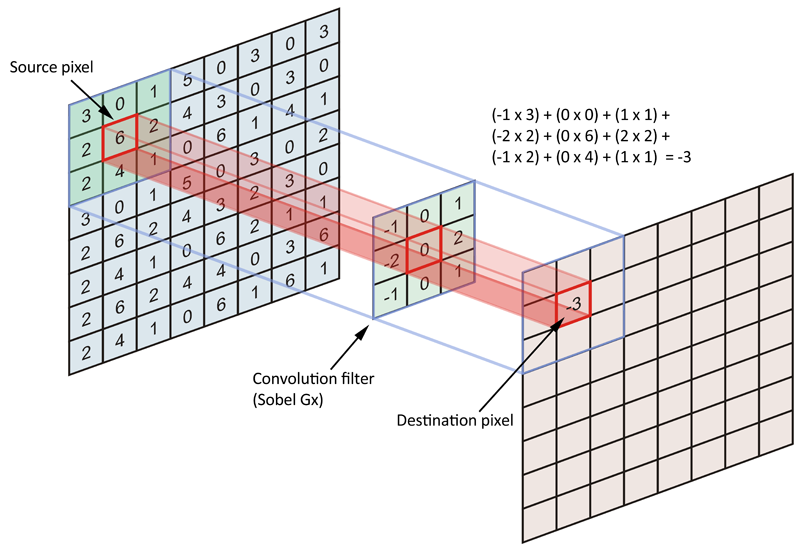
\includegraphics[scale=0.28]{./images/kernel_convolution}
				\end{figure}
		\end{frame}	

%Frame----------------------------------------------------------------------------------------------------------------------------------------------------
		\begin{frame}{XCA - IFCA Engine }
\begin{block}{Use CA instead of normal IP tecniques to get parallelism transparently!}
\end{block}		
		

		\begin{itemize}
			\item Implemented on top of \textbf{OpenCAL}
			\item Each color channels is represented as a substate
			\item Local and Global Pixel transformations maps directly to \textit{elementary processes} and \textit{global operations}, respectively.
			\item Runs on a number of parallel architectures and accelerators
			\item Easy to use. Threshold Filter in ~$20$ LoC.
			\item Seamless input/output
			\end{itemize}
		\end{frame}
		%Frame----------------------------------------------------------------------------------------------------------------------------------------------------
		\begin{frame}[fragile]{XCA - IFCA Engine}
			 \begin{lstlisting}[language=C,basicstyle=\tiny\ttfamily]
template<uint DIM, class NEIGH, typename CT, class PT>
class ThresholdFilter : public opencal::CALLocalFunction< DIM , NEIGH , CT>{

    TYPE lowT , highT ;
    TYPE outRangeValue , inRangeValue;

    ThresholdFilter(auto* sbs, TYPE _lowT , TYPE _highT , TYPE _outrange, TYPE _inrange ):
        img(sbs), lowT(_lowT) , highT(_highT) , 
        outRangeValue(_outrange) , inRangeValue(_inrange) { }
    
    void run(MODELTYPE* model,std::array<CT,DIM>& indices){
        
        constexpr int channels = std::tuple_size<PT>::value;
        PIXELTYPE newVal=img->getElement(indices);

        for (int i = 0; i<channels; ++i){
            const TYPE output =  (newVal[i] >= lowT && newVal[i] <= highT) ?
            					 inRangeValue : outRangeValue ;
            newVal[i] = output;
        }
        img->setElement(indices,newVal);
    }
};			
			
	\end{lstlisting}
		\end{frame}		
		
	
%Frame----------------------------------------------------------------------------------------------------------------------------------------------------
		
	\section{Tracking Algorithm}
%Frame----------------------------------------------------------------------------------------------------------------------------------------------------	
		\begin{frame}{Objective}
			\begin{block}{Problem tackled}
				From a time ordered sets of particles, output individual trajectories. 
\begin{itemize}
	\item Particles are described by a centroid and a bounding
box
\item Bounding box describes geometrical properties of the object
(shape area/volume etc.)
\item The algorithm is based on centroid/shape minimization
difference method
\end{itemize}
			\end{block}
	        \end{frame}
        
        

%Frame----------------------------------------------------------------------------------------------------------------------------------------------------

        \begin{frame}

			A \textit{distance} function must be defined for the particular particle representation. 
			\[
			\mathcal{D} : P \times P \mapsto R
			\]
$\mathcal{D}(p, q)$ measures the likeliness that
a particle p has been transformed into q as a result of the
application of a number of geometrical transformations such
as translation, scaling, shearing or rotation	


		\begin{figure}
					\centering
					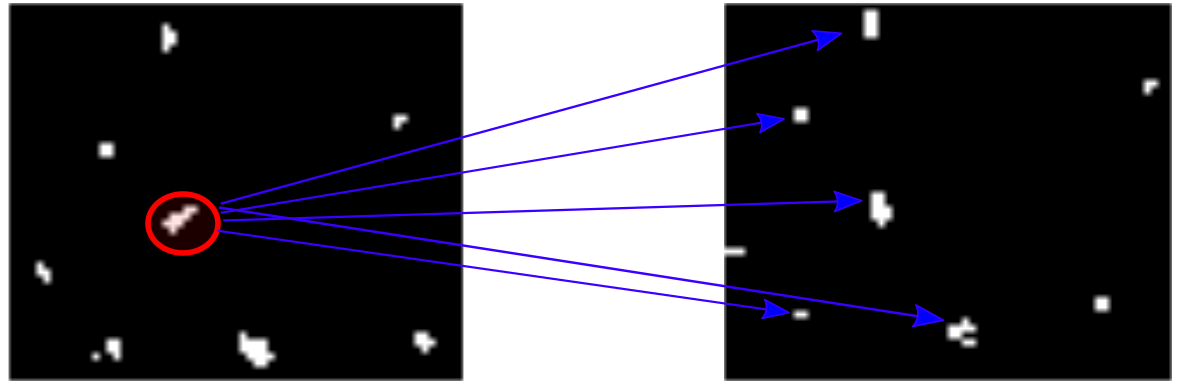
\includegraphics[scale=0.20]{./images/freccia.png}
					\caption{Distance function is computed for each particle between two subsequent frames.}
				\end{figure}
			\end{frame}
	
	%Frame----------------------------------------------------------------------------------------------------------------------------------------------------
\begin{frame}
 \begin{block}{Algorithm Formalization} 
Let $P = P_1  \union P_2 \union \ldots \ P_n$ be the set of frames, $\mathcal{D} : P \times P \mapsto\mathbb{R}$ the distance function. $P_i = \{p_i^j | 1 \leq j \}$ indicates all particles at time $i$. Iteratively processes at each step two set $M_i$ and $P_i$. $M_i$ is the set of \textit{under construction} trajectories.

\begin{itemize}
	\item It augment an element of $M_i$ using a 	particle at
	frame $i+1$ s.t. the distance function is 			minimized.
	\end{itemize}
\end{block}


.\end{frame}       
	
			
\begin{frame}{Objective}
		
\begin{columns}[T] % align columns
\begin{column}{.40\textwidth}

\hfill \\ \hfill
\hfill \\ \hfill
\[
\forall (u,v) \in S 
\]

\[
\left\{
  \begin{array}{lr}
   (w,x) \in S,\; v=x\Longleftrightarrow u=w\\
   \mathcal{D}(u,v) = \min_{x \in V_2} \mathcal{D}(u,x)  \\
    \nexists \: (w,v) \in E \: \mbox{s.t.} \: \mathcal{D}(w,v) < \mathcal{D}(u,v)
  \end{array}
\right.
\label{matchConstraints}
\]
Invariants that the algorithm forces on the solution
\end{column}%
\hfill%
\begin{column}{.48\textwidth}


		\begin{figure}
					\centering
					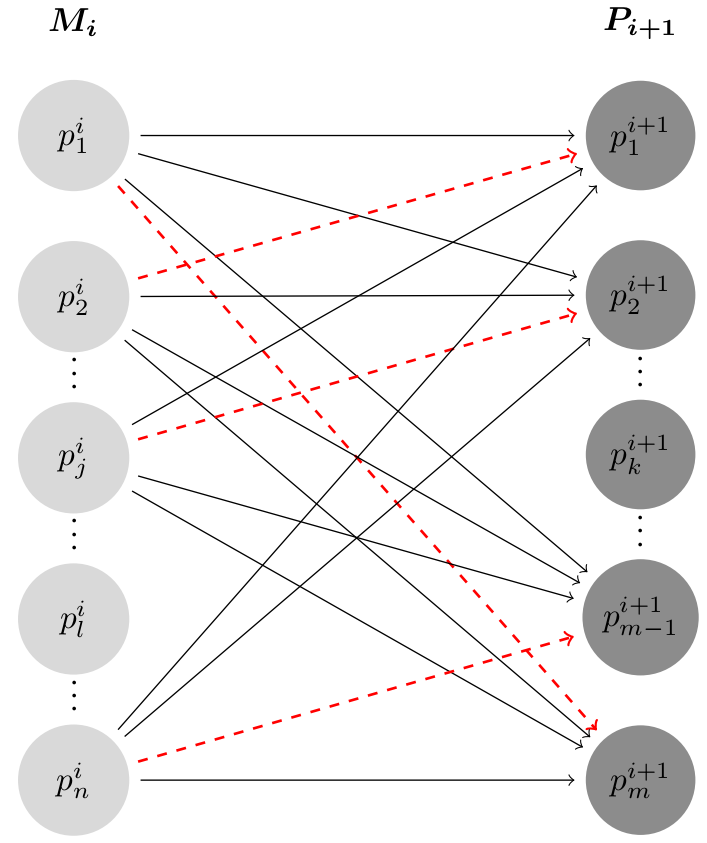
\includegraphics[scale=0.19]{./images/graph.png}
					
				\end{figure}
\end{column}%
\end{columns}
\end{frame}
	

			
			
			
	

	



\section{Test Case: Motility of B. Subtilis}

%Frame----------------------------------------------------------------------------------------------------------------------------------------------------
	\begin{frame}{}
		\begin{block}{How bacteria move}
			
			\begin{itemize}
				\item \textit{run} is a swim along a smooth segment
				\item tumble is a stop plus a change in direction (in \textit{random} fashion) 
			\end{itemize}
		\end{block}
		
		\begin{figure}
					\centering
					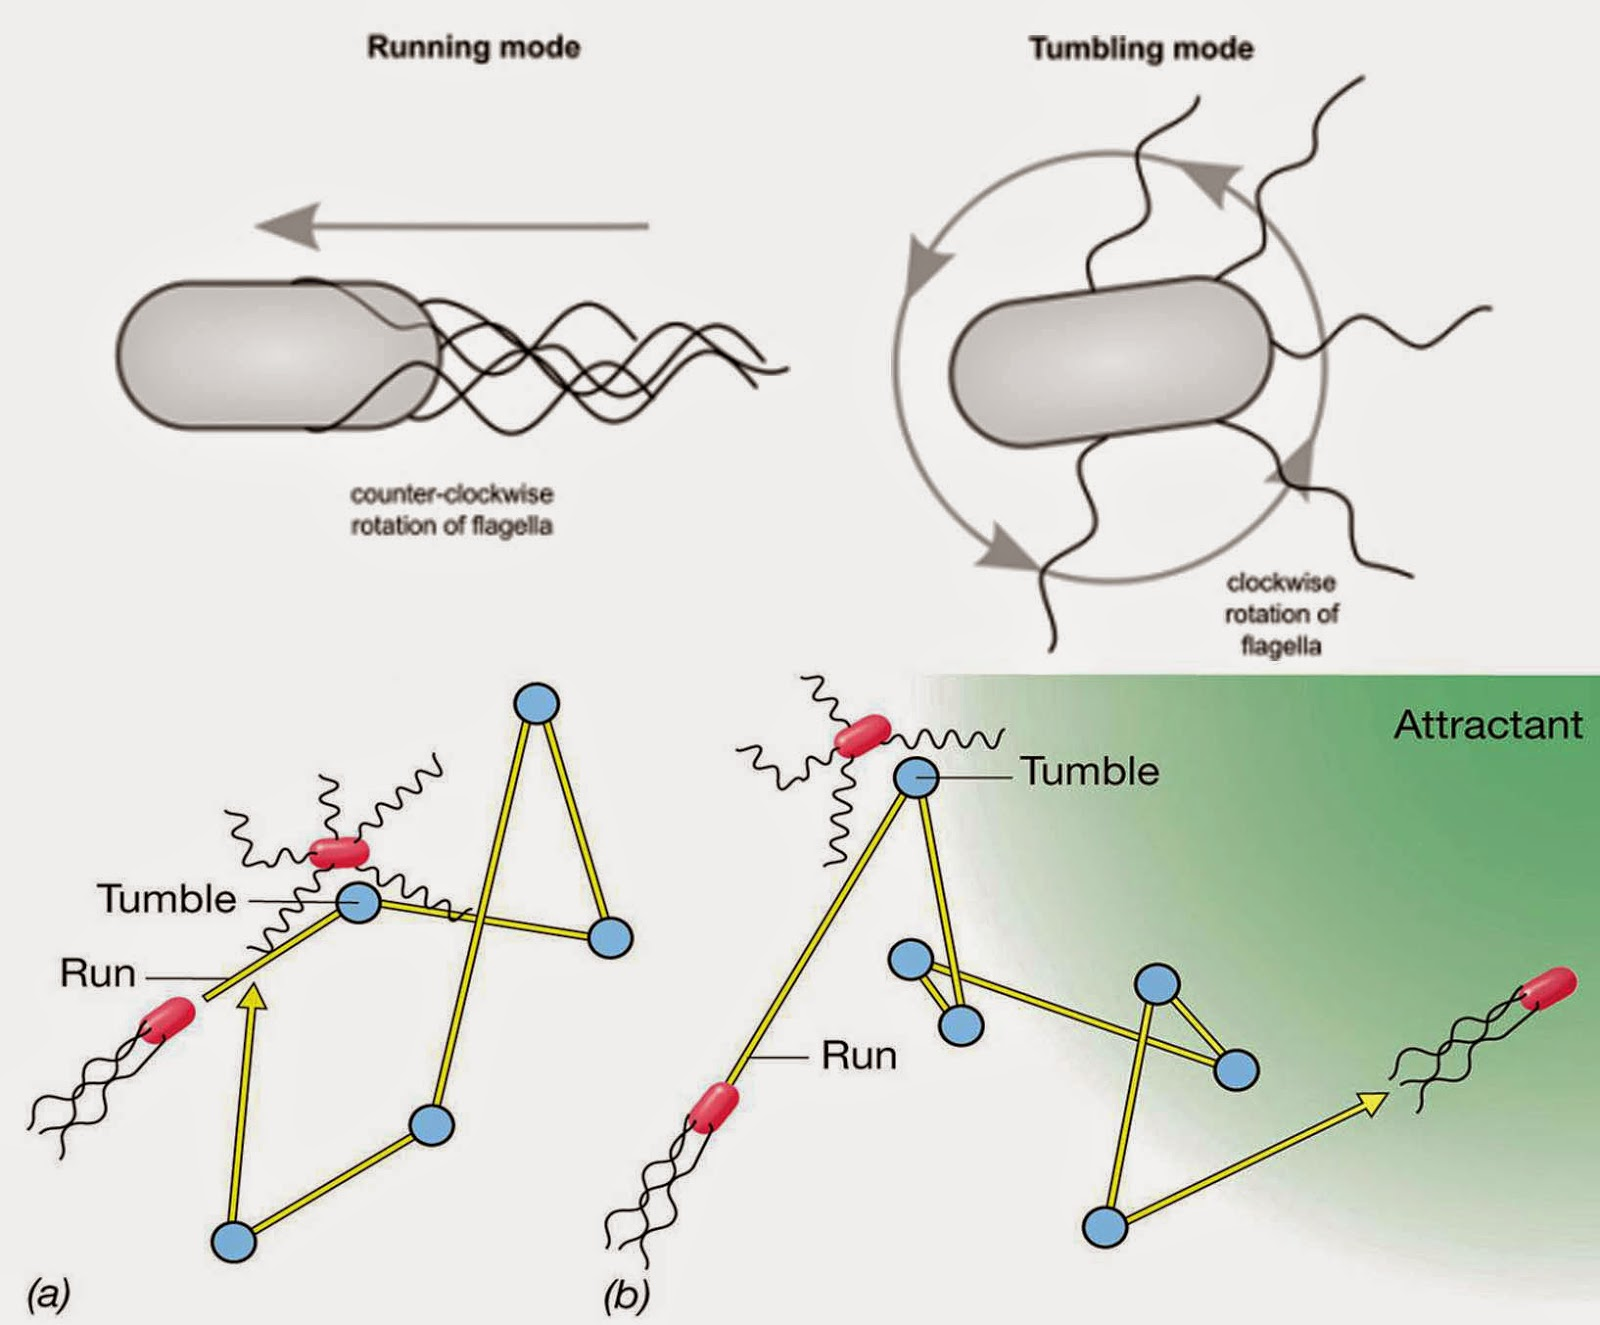
\includegraphics[scale=0.10]{./images/run}
				\end{figure}

	\end{frame}
%Frame----------------------------------------------------------------------------------------------------------------------------------------------------
	\begin{frame}{Experiment Setting}
\begin{itemize}
\item B. subtlis \texttt{OI1085} from frozen, resuspended in CAM and shaken.
\item Solution is injected in microfluidic device (PDMS and glass made of 3 channels height 100 $\mu$m)
\item Pictures taken at 100 frames per second
\item Nikon Microscope 10X phase contrast  $2 \times 2$ binning
\end{itemize}
	\end{frame}
	

%Frame----------------------------------------------------------------------------------------------------------------------------------------------------

\begin{frame}{Input Preprocessing}
				\begin{itemize}
					\item Raw images pass through a pipeline of filters which eventually segments particles from the background
					\item The pipeline is composed by a \textbf{contrast stretch} , \textbf{gaussian}, \textbf{laplacian }and \textbf{blurring filters}.
					\item Filters are applied in a data parallel way on a single image.
					\item Multiple images filtering is emberassingly parallel.
				\end{itemize}
	\end{frame}

	
%Frame----------------------------------------------------------------------------------------------------------------------------------------------------
	\begin{frame}{Input Preprocessing}
				\begin{figure}
					\centering
					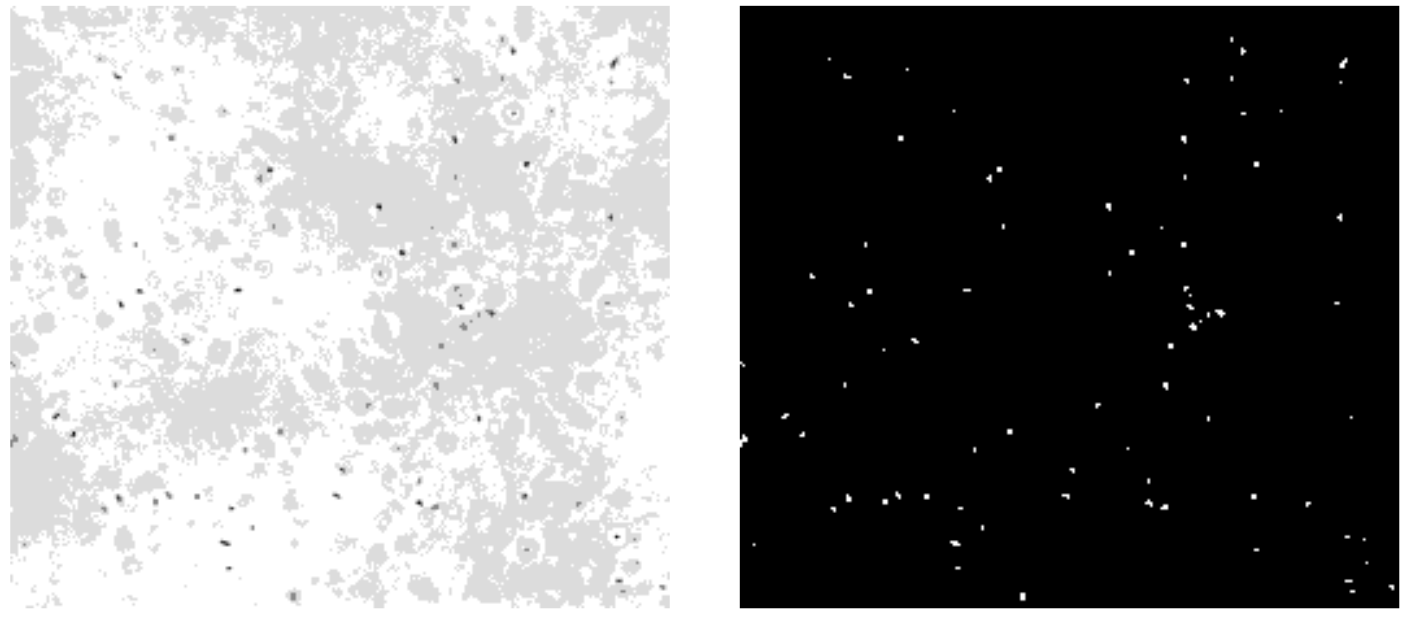
\includegraphics[scale=0.20]{./images/preproc}
					\caption{Raw data on the left and the processed image on the right.}
				\end{figure}
	\end{frame}
	%--------------------------------------------------------------------------------------------------------------------


%Frame----------------------------------------------------------------------------------------------------------------------------------------------------
	\begin{frame}{Tracking of B. subtilis}
				\begin{itemize}
					\item Finally, centroids and bounding boxes are extracted
					\item Centroid is represented by a pair double precision number
					\item Bounding box and shape difference is managed by the \textit{CGAL} library
					\item Distance function: 
					\begin{equation}
\label{sec:bacttracking}
D(c_i,c_j) = a \sqrt{(x_{c_i} - x_{c_j})^2 + (y_{c_i}-y_{c_j})^2} + b |S_i \cap S_j|
\end{equation}
is linear combination of centroid distance and shape difference.
\item Weights $a=0.6$ and $b=0.4$ 
					\end{itemize}
	\end{frame}
	

\subsection{Validation}

%________________________frame

\begin{frame}
Trajectories have been post-processed dividing them  in a list of running and tumbling events.
		\begin{figure}
					\centering
					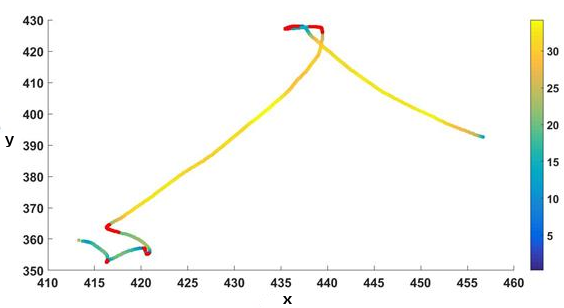
\includegraphics[scale=0.40]{./images/runtumble.png}
					
\end{figure}


				

\end{frame}


\begin{frame}
\begin{center}
Then the following metrics have been used to validate the proposed method:
\begin{center}
	\begin{itemize}
		
		\item \textbf{Mean Swimming Time}
		\item \textbf{Mean Run Time}
		\item \textbf{Tumble Time}
	\end{itemize}
\end{center}
Results are in accordarnce those presented in literature (see \textit{Cisneros et al})


\end{center}
\end{frame}



\begin{frame}
\begin{center}
\begin{figure}
	\centering
					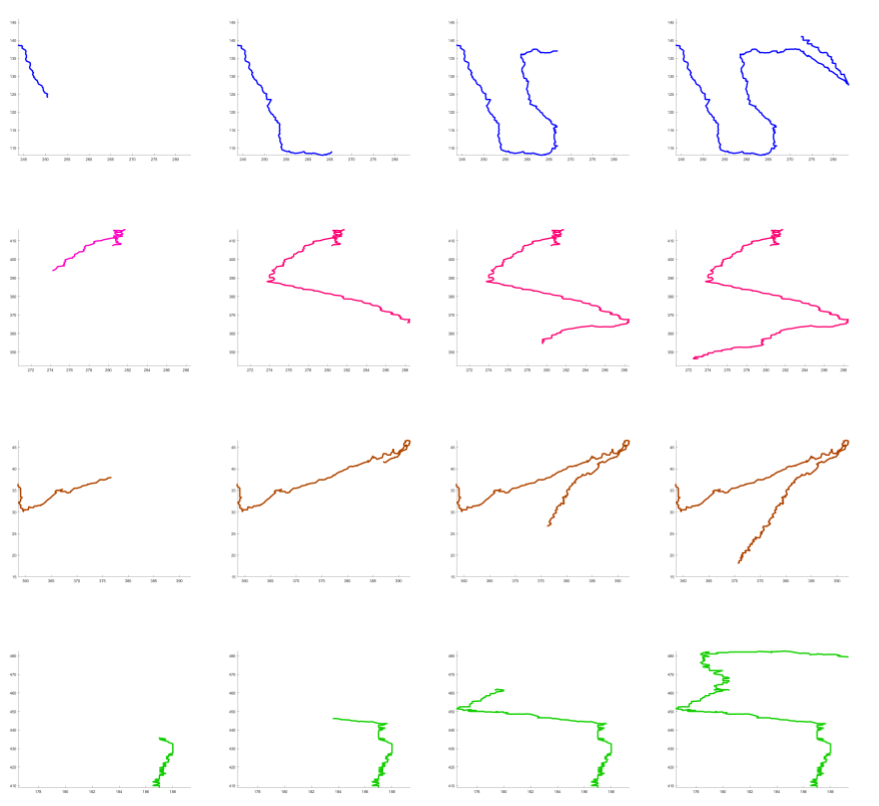
\includegraphics[scale=0.25]{./images/traj.png}
					
\end{figure}

\end{center}
\end{frame}

\begin{frame}
\begin{center}
\centering
\fbox{	
	\movie[width=6cm,height=6cm,autostart,loop,poster,palindrome]{}{output.mp4}}
				


\end{center}
\end{frame}


\begin{frame}
\begin{center}
{\fontsize{40}{50}\selectfont Thank You!}
\end{center}
\end{frame}

\end{document}